\documentclass[aspectratio=169, 11pt]{beamer} % aspectratio=43, 149, 169
% 余分なオプションを削除しました。aspectratioはそのままで大丈夫です。

% 必要なパッケージを読み込みます
\usepackage{amsmath, amssymb, bm, mathtools, multicol, tcolorbox, subfig, physics, ulem, url}
\usepackage{here} % 'here' パッケージは推奨されていない場合があるので注意
\usepackage{ascmac, array}

% Beamerテーマとカラーテーマ
\usetheme{Berlin}
\usecolortheme[RGB={4, 56, 76}]{structure}
\usefonttheme{professionalfonts}
\useinnertheme{circles}
\useoutertheme{infolines}


\setbeamertemplate{bibliography item}[text]

% ナビゲーションシンボルを非表示に
\setbeamertemplate{navigation symbols}{}

% タイトルとフレームタイトルの色設定
\setbeamercolor{title}{fg=structure, bg=}
\setbeamercolor{frametitle}{fg=structure, bg=}

% itemizeの設定
\setbeamertemplate{itemize item}{\small\raise0.5pt\hbox{$\bullet$}}
\setbeamertemplate{itemize subitem}{\tiny\raise1.5pt\hbox{$\blacktriangleright$}}
\setbeamertemplate{itemize subsubitem}{\tiny\raise1.5pt\hbox{$\bigstar$}}

\usepackage{fontspec}
\usepackage{luatexja-fontspec}

\setsansfont{Helvetica} % 英語用のサンセリフフォント
\setmainjfont{Hiragino Kaku Gothic ProN} % 日本語用のゴシック体フォント
\setsansjfont{Hiragino Kaku Gothic ProN} % 日本語用のサンセリフ(ゴシック体)フォント



% カラーのショートカット
\newcommand{\red}[1]{\textcolor{red}{#1}}
\newcommand{\green}[1]{\textcolor{green!40!black}{#1}}
\newcommand{\blue}[1]{\textcolor{blue!80!black}{#1}}

% 数学的なコマンド
\newcommand{\R}{\mathbb{R}}
\newcommand{\Z}{\mathbb{Z}}
\newcommand{\N}{\mathbb{N}}
\newcommand{\C}{\mathbb{C}} 

% タイトル情報
\title[]{Reservoir Computerによる外力付きカオス時系列モデルの予測と生体リズム研究への応用}
\subtitle{}
\author[]{発表者:久野 証\\指導教官:郡 宏教授}
\institute[]{所属:東京大学工学部計数工学科数理情報工学コース 4年\\学籍番号:03-210599}
\date{\today}

% ドキュメントの開始
\begin{document}
    \maketitle
    % ここにスライドの内容を追加

    \begin{frame}{目次}
        \tableofcontents
    \end{frame}  

    \section{背景}
\begin{frame}{LD Cycleによる生体リズムの研究}
        \begin{block}{概日リズムの研究:LD Cycle}
          \begin{itemize}
            \item 時差ぼけやシフトワークは、生活習慣病のリスクを高める.
            \item LD Cycleは生体リズムのモデルに用いられ,光と暗闇の情報が外力として系に加わる.\begin{itemize}
              \item 時差ぼけ/シフトワークの研究では,この外力の位相をシフトさせることを考える.
            \end{itemize}
            \item 外力や各パラメータの設定により周期的・カオス的な振る舞いを持つ.
            \item 一般にカオスの予測は難しい(初期値鋭敏性).
          \end{itemize}
        \end{block}
        \vspace{-.5em}
        \begin{figure}
          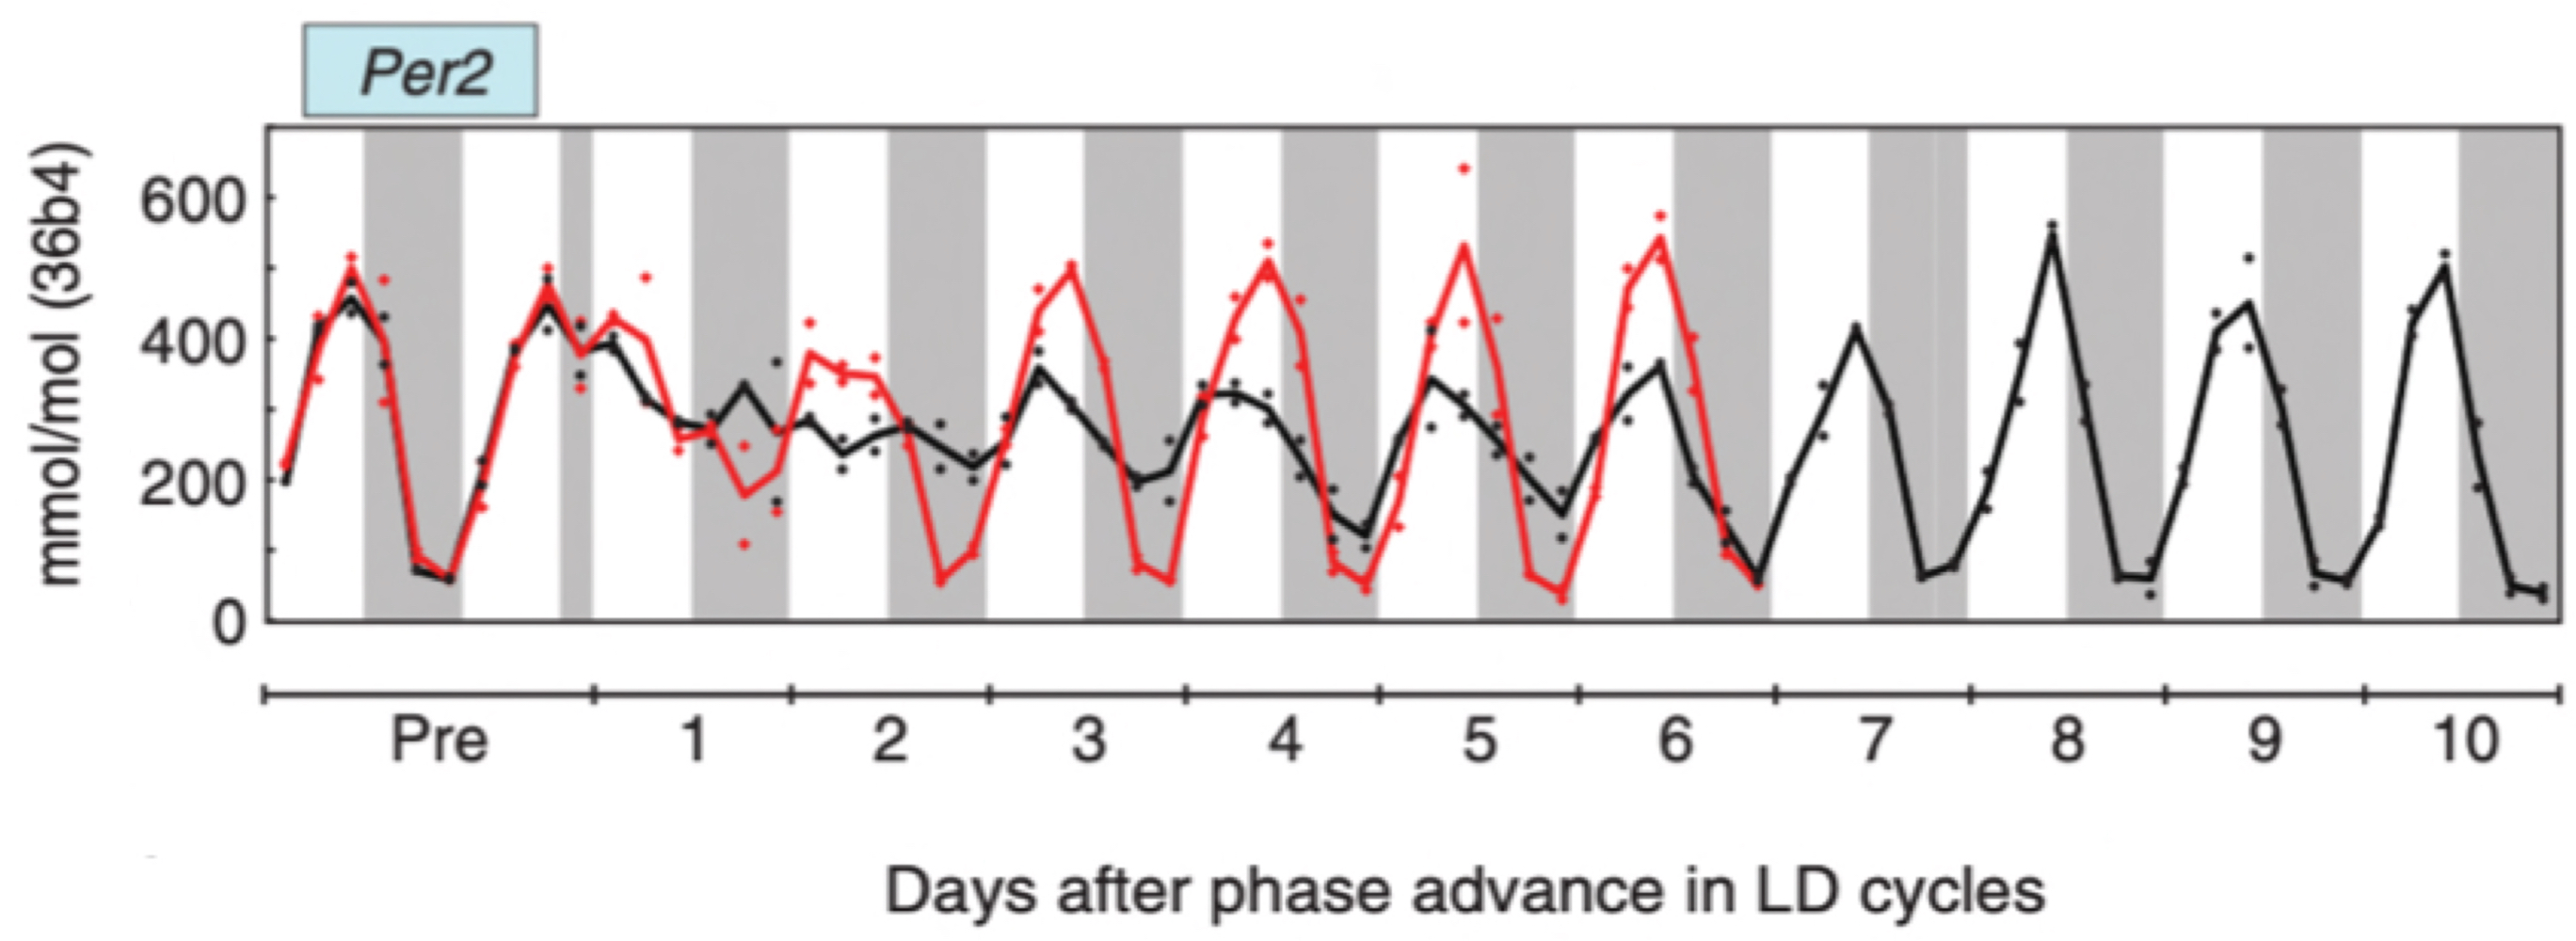
\includegraphics[width=0.4\textwidth]{Fig/Jetlag.png}
          \caption{\scriptsize{Day 1に8時間のJet Lagを受けた時のマウスの Per2 の推移}\\\tiny{Image: Fig.2 from \cite{Yamaguchi et al.}.}}
      \end{figure}    
      
  \end{frame}

  \section{手法}

\begin{frame}{Reservoir Computer の特徴}
    % スライドを2つの列に分割
    \begin{columns}[T] % [T] は列を上部で揃えるオプション
  
      \begin{column}{.5\textwidth}
        
        \begin{itemize}
          \item 右側のアイテム1
          \item 右側のアイテム2
        \end{itemize}
      \end{column}

      \begin{column}{.5\textwidth}
        \begin{figure}
            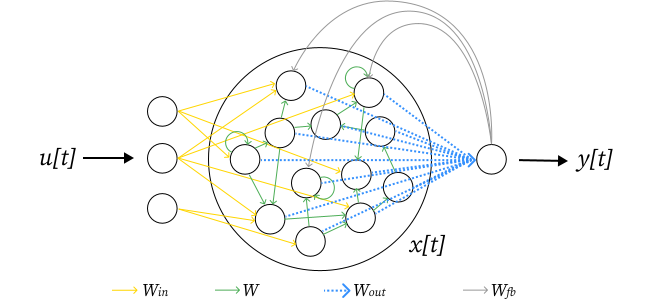
\includegraphics[width=\textwidth]{Fig/esn.svg.png}
        \end{figure}  
        \begin{figure}
            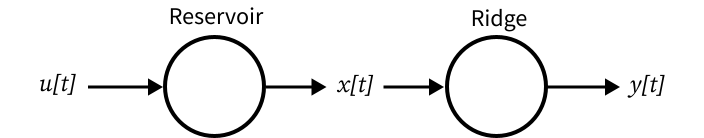
\includegraphics[width=\textwidth]{Fig/esn_nodes.svg.png}
            \caption{\scriptsize{Reservoirpy での reservoir computer の構造}\\ \tiny{Image: ReservoirPy, MIT License.}}
        \end{figure}  
      \end{column}
    \end{columns}
  \end{frame}



    \begin{frame}{周期外力のあるRösslerモデル (1/2)}
    \vspace{-.35cm}
    % スライドを2つの列に分割
    \begin{columns}[T] % [T] は列を上部で揃えるオプション
  
      \begin{column}{.5\textwidth}
        \begin{block}{Rössler方程式}
            次の方程式を解くことで時系列データを生成する.
            \begin{align}
                \frac{dx}{dt} &= -y - z + P(t)\\
                \frac{dy}{dt} &= x + ay \\
                \frac{dz}{dt} &= b + z(x - c)
            \end{align}
            ここで,$P(t) := A \sin(t + \theta_p(t))$ とする.
           
            ただし,$p \in \left\{ n \in \Z \mid -12 \leq n \leq 12 \right\}$ とし,
            $\theta_p$ は $4$ 日に $1$ 度外力の位相を $p\cdot 2\pi/24$ だけ早めるような関数.
        \end{block}
      \end{column}
      \begin{column}{.5\textwidth}
        \vspace{-.6cm}
        \begin{figure}
            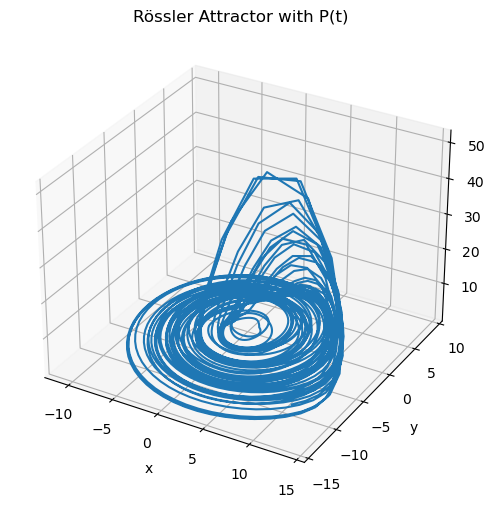
\includegraphics[width=0.9\textwidth]{Fig/NEWrossler_attractor.png}
            \caption{\scriptsize{Rösslerモデル}}
        \end{figure}
        
      \end{column}
    \end{columns}
  \end{frame}

\begin{frame}{周期外力のあるRösslerモデル (2/2)}
    \begin{columns}[T] % [T] は列を上部で揃えるオプション
        \begin{column}{.5\textwidth}
            \begin{itemize}
                \item Hyperparameter の最適化は位相シフトが$8$時間である系に対して行う.
                \item その後,同じ Reservoir で異なる位相シフトを持つ系に対しても予測を行う.\begin{itemize}
                    \item 未知の外力に対するReservoir の予測性能を測る.
                \end{itemize}
            \end{itemize}
            
            \vspace{-.5em}
            \begin{figure}
                %\centering % 画像を中央揃えにする(オプション)
                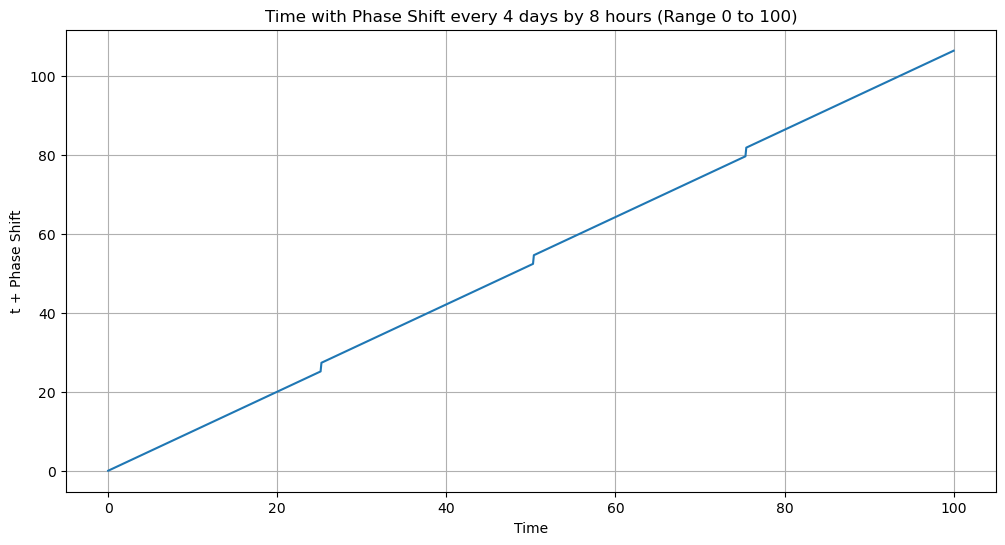
\includegraphics[width=0.8\textwidth]{Fig/phase_shift_plot.png}
                \caption{\scriptsize{$4$ 日に一度 $8$ 時間早めたときの外力の位相}}
            \end{figure}
        \end{column}
        \begin{column}{.5\textwidth}
            \vspace{-1cm}
            \begin{figure}
                %\centering % 画像を中央揃えにする(オプション)
                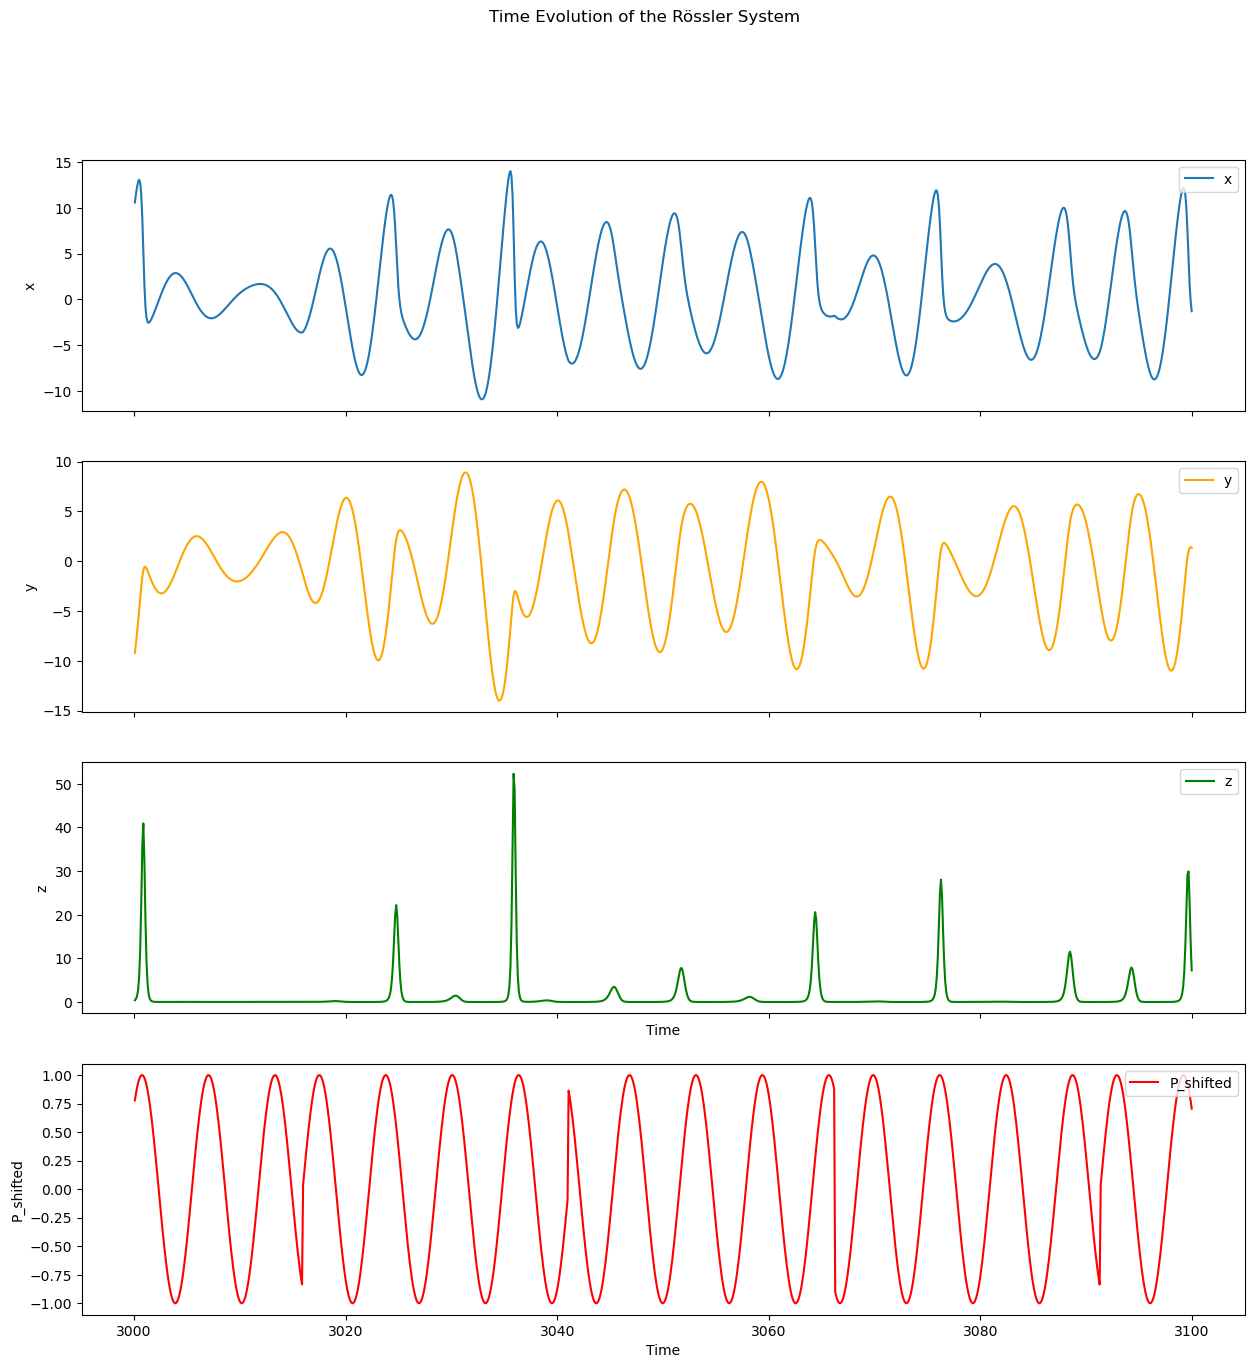
\includegraphics[width=0.8\textwidth]{Fig/NEWrossler_waves.png}
                \caption{\scriptsize{位相シフトのある周期外力付きのRössler システム:\\
                上から $x, y, z, P(t)$. }}
            \end{figure}
        \end{column}
      \end{columns}
    
\end{frame}


\section{結果}
\begin{frame}
    
\end{frame}

\section{まとめと展望}
\begin{frame}
    
\end{frame}

    \documentclass[../main]{subfiles}
\begin{document}
\chapter{鎖状ネットワークの同期に関する先行研究}
\label{chap:appendix}
\cite{XiaHuang:130506}の解析内容について述べる.\\
鎖状に無向グラフとして$N$個連なった位相振動子ネットワークのふるまいを以下で記述するとする.
\begin{align*}
    \dot{\theta}_1&=\omega_1\\
    \dot{\theta}_i&=\omega_i+\lambda\sin(\theta_{i-1}-\theta_i),\ i=2,3,\ldots,N
\end{align*}
ここで,$\theta_i,\omega_i$をそれぞれ端から$i$番目の振動子の位相と固有振動数とする.$\lambda>0$は振動子間の結合強度とする.
このモデルでは端の振動子$1$が固有振動数$\omega_1$をもつ駆動源となり,他の振動子は駆動源に近い方の隣接した振動子と相互作用する.\\

$\omega_1=2,\omega_2=1$とし,他の$\omega_i$をランダムに選択するとして固有振動数を配置し,結合強度を高めていく数値実験を行ったところ,4つのクラスタリングパターンが観測された.
\renewcommand{\labelenumi}{Case  \theenumi}
\begin{enumerate}
    \item \label{enu:case1} 隣接した駆動振動子と同期し局所クラスターが発生する.
    \item \label{enu:case2} 駆動源と同期する振動子が出現する.
    \item \label{enu:case3} 結合強度が小さい間は隣接した駆動振動子と同期し局所クラスターを構成した後,結合強度がある程度大きくなると局所クラスターが消滅する.
    \item \label{enu:case4} 隣接した駆動振動子が駆動源と同期した後,駆動される振動子自体も同期する.
\end{enumerate}
つまり,各振動子とクラスターを構成するのは,隣接した駆動振動子と,駆動源の2つの振動子のみである.
このパターンは,他の鎖状ネットワークでも普遍的であるため,これらのクラスタリングパターンの分岐を考える.

特に$N=3,\ \omega_1=2,\ \omega_2=1$とする.$\omega_3$を変化させたとき全部で4つの領域に分かれた.
\begin{itemize}
    \item $\omega_3\in[1,2]$のとき,結合強度の増加により隣接した駆動振動子と同期する.Case \ref{enu:case1}に相当する.
    \item $\omega_3\in(2,3]$のとき,結合強度の増加により駆動振動子と同期する.Case \ref{enu:case2}に相当する.
    \item $\omega_3\lesssim 1$のとき,結合強度が小さい間は隣接した駆動振動子と同期し局所クラスターを構成した後,結合強度がある程度大きくなると局所クラスターが消滅する.Case \ref{enu:case3}に相当する.
    \item $\omega_3$が$\omega_1,\omega_2$両方ともから離れた値のとき,隣接した駆動振動子が駆動源と同期した後,駆動される振動子自体も同期する.Case \ref{enu:case4}に相当する.
\end{itemize}
以上の分岐を調べるため,以下の方程式を考える.
\begin{align}
    \label{eq:3driving}
    \begin{split}
        \dot{\theta}_1&=\omega_1\\
        \dot{\theta}_2&=\omega_2+\lambda\sin(\theta_1-\theta_2)\\
        \dot{\theta}_3&=\omega_3+\lambda\sin(\theta_2-\theta_3)
    \end{split}
\end{align}
ここで,$\phi_{21}=\theta_2-\theta_1,\ \Delta\omega_{21}=\omega_2-\omega_1$とすると,
\begin{align}
    \label{eq:phasediff-21}
    \dot{\phi_{21}}=\Delta\omega_{21}-\lambda\sin\phi_{21}
\end{align}
となる.ここで,両辺の長時間平均$\langle\cdot\rangle$を考える.
$\lambda$が同期が起こらないくらい小さいとき,$\phi_{21}$の確率分布$\rho(\phi_{21},t)$は十分時間が経つと安定分布に収束する.
\begin{align*}
    \rho(\phi_{21},t)=\frac{\Delta\omega_{21}-\lambda\sin\phi_{21}}{C},\quad C:\mathrm{normalization\ constant}
\end{align*}
この確率分布に$\phi_{21}$が従うとして式\eqref{eq:phasediff-21}の$\sin\phi_{21}$を平均する.
すると,
\begin{align*}
    \langle\sin\phi_{21}\rangle=\frac{\Delta\omega_{21}-\sqrt{(\Delta\omega_{21})^2-\lambda^2}}{\lambda}
\end{align*}
よって,式\eqref{eq:3driving}より,$\theta_2$の実効振動数が得られる.
\begin{align*}
    \langle\dot{\theta}_2\rangle=\omega_1+\sqrt{(\Delta\omega_{21})^2-\lambda^2}
\end{align*}
この式より,$\lambda_c=\Delta\omega_{21}$として,$\lambda\geq\lambda_c$のとき$\langle\dot{\theta}_2\rangle=\omega_1$となり,振動子$1$と振動子$2$は同期する.
同様の手順で$\theta_3$の実効振動数が得られる.
\begin{align}
    \label{eq:effective-approx}
    \langle\dot{\theta}_3\rangle=\langle\dot{\theta}_2\rangle+\sqrt{(\Delta\omega_{32})^2-\lambda^2}
\end{align}
ただし,$\Delta\omega_{32}=\omega_3-\langle\dot{\theta}_2\rangle$である.\\
以上より,振動子の同期条件を求めることができる.
振動子$2$と振動子$3$の同期条件は
$\Delta\omega_{21}\geq 0$のとき,
\begin{align*}
    \begin{cases}
        -\lambda\leq\Delta\omega_{31}-\sqrt{(\Delta\omega_{32})^2-\lambda^2}\geq\lambda & (\lambda\leq|\Delta\omega_{21}|)\\
        -\lambda\leq\Delta\omega_{31}\geq\lambda & (\lambda>|\Delta\omega_{21}|)
    \end{cases}
\end{align*}
$\Delta\omega_{21}< 0$のとき,
\begin{align*}
    \begin{cases}
        -\lambda\leq\Delta\omega_{31}+\sqrt{(\Delta\omega_{32})^2-\lambda^2}\geq\lambda & (\lambda\leq|\Delta\omega_{21}|)\\
        -\lambda\leq\Delta\omega_{31}\geq\lambda & (\lambda>|\Delta\omega_{21}|)
    \end{cases}
\end{align*}
ここで,$\Delta\omega_{31}=\omega_3-\omega_1$である.
これらの同期条件から,$\omega_c=-\sqrt{2}|\Delta\omega_{21}|+\omega_1$という臨界振動数を境界とする領域$\omega_3\in(\omega_c,\omega_2)$でCase \ref{enu:case2}のような分離が起こることがわかる.\\
次に,振動子$1$と振動子$3$の同期条件を考える.
$\phi_{31}=\theta_3-\theta_1$とすると,
\begin{align*}
    \dot{\phi}_{31}=\Delta\omega_{31}-\lambda\sin(\phi_{31}-\phi_{21})
\end{align*}
となるから同期の必要条件は,$|\Delta\omega_{31}|\leq \lambda$となる.
また,$\langle\dot{\theta}_3\rangle=\omega_1$の状況を考えると,式\eqref{eq:effective-approx}から,同期の十分条件が求まる.
\begin{align*}
    \omega_3\leq\omega_1+|\Delta\omega_{21}|-\sqrt{(\Delta\omega_{21})^2-\lambda^2}
\end{align*}
以上の解析から$\omega_3,\lambda$と同期クラスタの関係が図\ref{fig:appendix-bifurcation}として示される.
\begin{figure}[t]
\centering
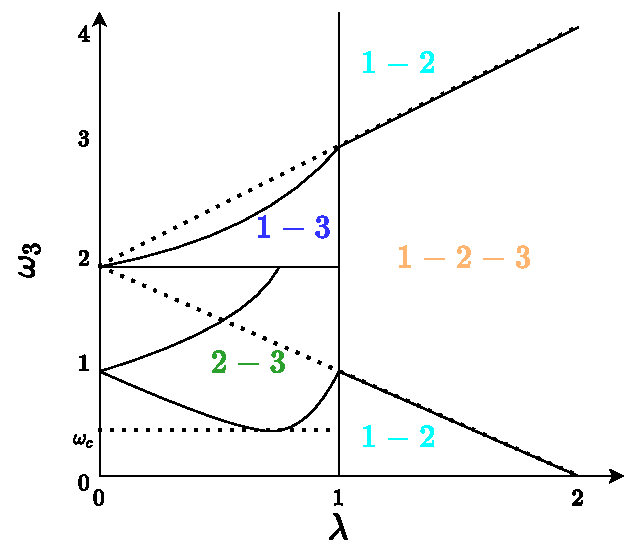
\includegraphics[width=70mm]{./images/appendix-bifurcation.pdf}
\centering
\caption{$\omega_1=2,\ \omega_2=1$のときの固有振動数$\omega_3$と結合強度$\lambda$に対する相図.
あるパラメータ領域で同期クラスタが発生する場合,その振動子の組を各領域に示している.また,同期クラスタが異なるパラメータ領域の境界を実線で示している.}
\label{fig:appendix-bifurcation}
\end{figure}
また,式\eqref{eq:effective-approx}を再帰的に利用することで$N>3$の場合でも同様の解析が可能となる.
\end{document}

\end{document}
